\chapter{Single dimension model combination\label{sec:combination}}\thispagestyle{empty}
In chapter \ref{sec:singleDimension}, the construction of single dimension models is discussed.
These models extimate the segmentation masks of $352 mm\times 352 mm$ patches of scan volume slices along one of the three main axis.
In this chapter, the results of these single dimension models are combined to form a \textit{pseudo} mask that is subsequently used as labelling to train the final segmentation network.
Details regarding this combination procedure are given on page \pageref{sec:combinationProcedure}.
Interesting to note in this procedure is that the evaluation metric of these obtained segmentation masks is improved in each of these steps.
The pseudo mask volume performs better than the single dimension model results and the final model trained on the pseudo masks performs better than the pseudo mask itself. 

\begin{SCtable}[\sidecaptionrelwidth][h]

    \begin{tabular}{l|lll}
        \hline
        \textbf{\begin{tabular}[c]{@{}l@{}}Slice \\ direction\end{tabular}} &
          \textbf{Transverse} &
          \textbf{Coronal} &
          \textbf{Sagittal} \\ \hline
        \begin{tabular}[c]{@{}l@{}}Context\\ Slices {[}mm{]}\end{tabular}           & 1      & 1      & 1      \\ \cline{1-1}
        \begin{tabular}[c]{@{}l@{}}Points per\\ class instance\end{tabular}         & 1      & 1      & 1      \\ \cline{1-1}
        \begin{tabular}[c]{@{}l@{}}Background \\ points\end{tabular}                & 5      & 3      & 3      \\ \cline{1-1}
        Dataset &
          \begin{tabular}[c]{@{}l@{}}PLoS\\ xVertSeg\\ USiegen\\ MyoSegmenTUM\end{tabular} &
          \multicolumn{2}{l}{\begin{tabular}[c]{@{}l@{}}xVertSeg\\ USiegen\\ MyoSegmenTUM\end{tabular}} \\ \cline{1-1}
        \begin{tabular}[c]{@{}l@{}}Segmentation\\ classes\end{tabular}              & 2      & 6      & 6      \\ \cline{1-1}
        \begin{tabular}[c]{@{}l@{}}Weighted \\ dice score\end{tabular}              & 0.46   & 0.38   & 0.38   \\ \hline
        \begin{tabular}[c]{@{}l@{}}Weighted\\ dice score\\ combination\end{tabular} & \multicolumn{3}{c}{0.51} \\ \hline
        \end{tabular}
    \caption{Combination of three point supervised models with algorithm \ref{alg:combination}. 
    These models were constructed with a fixed number of background points and a fixed number of class labels per class instance.
    This test indicates that the segmentation mask obtained from the result of single dimension models with algorithm \ref{alg:combination} allows to obtain a new segmentation mask with a higher metric score, the pseudo masks.
    The weighted dice scores are evaluated on the cross validation set, this causes the difference with the values in figure \ref{fig:points_influence}. \label{tab:combination_1}
    }

\end{SCtable}
\par{
    In table \ref{tab:combination_1}, the segmentation quality is calculated on the validation set.
    Since there are two hyperparameters (the number of denoise iterations and the number of erosion iterations) to optimise in the combination algorithm \ref{alg:combination}, 
    the algorithm is evaluated with a matrix of these hyperparameters to choose the optimal hyperparameter set to construct the pseudo masks for the test set.
    In figure \ref{fig:hyperparameter_combination_1}, this obtimization procedure is illustrated.
    The optimal hyperparameter set in this case was 2 denoise iterations and 1 erosion iteration.
}
\marginpar{
        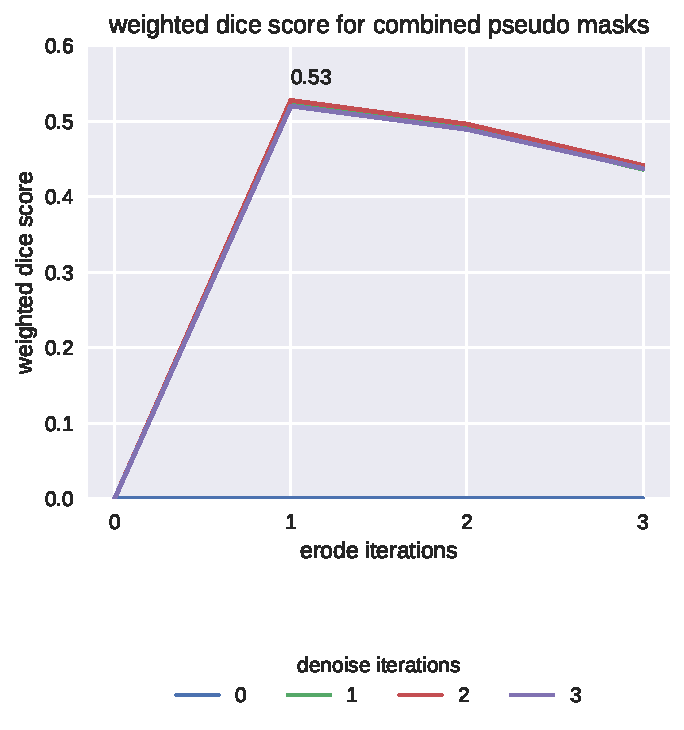
\includegraphics[width=5cm]{images/combination_optimization_1.pdf}
        \captionof{figure}{Illustration of the hyperparameter optimization procedure for the combination detailed in \ref{tab:combination_1}}
        \label{fig:hyperparameter_combination_1}
    }
\par{
    The result of this procedure is illustrated in figures \ref{fig:comb1_1}, \ref{fig:comb1_2} and \ref{fig:comb1_3}.
    These images illustrate that the result of the combination procedure is an improvement compared to the results of the individual models.
}   
\par{
    The procedure described in the last two chapters now allows to train a network with only point annotated labels by using the results of the pseudo mask volume.
    Mind however that the results in chapter \ref{sec:singleDimension} and the results combined in this chapter were obtained with a different set of point annotations for each dimension.
    This was done to make comparison possible.
}
\par{
    In reality, an expert will generate a single stack of annotations, not three.
    As described in chapter \ref{sec:annotationPoints} on page \pageref{sec:annotationPoints}, one of the single dimensional models will be trained on this stack of annotated slices.
    The other two however, will be trained on stacks where the same annotation points are used, but now as these are found back when slicing in the two other dimensions.
}

\begin{SCfigure}[][htb]
    \centering
    \centering
    \begin{minipage}{.99\textwidth}
        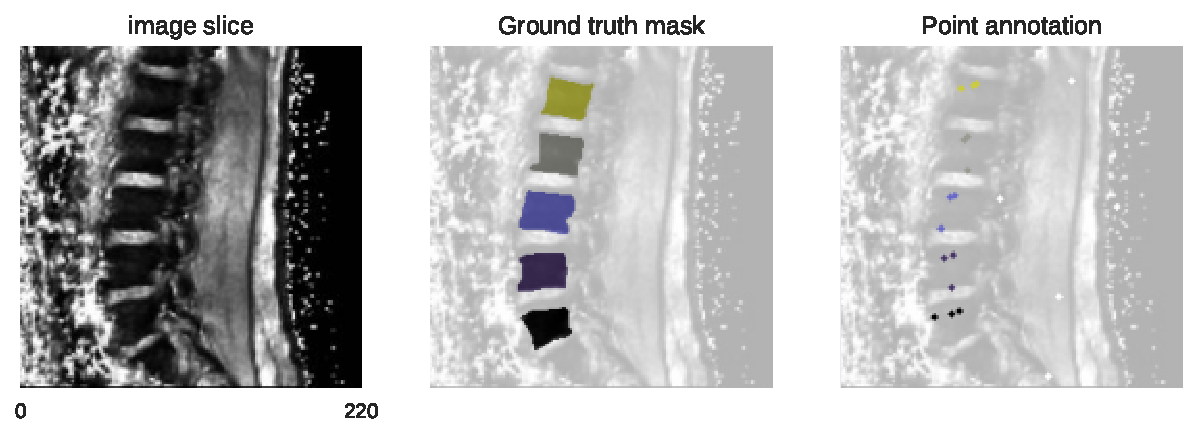
\includegraphics[width=.99\textwidth]{images/MyoSegmenTUM020_s21_points.pdf}
    \end{minipage} 
    \vspace{1 mm}
    \begin{minipage}{.99\textwidth}
        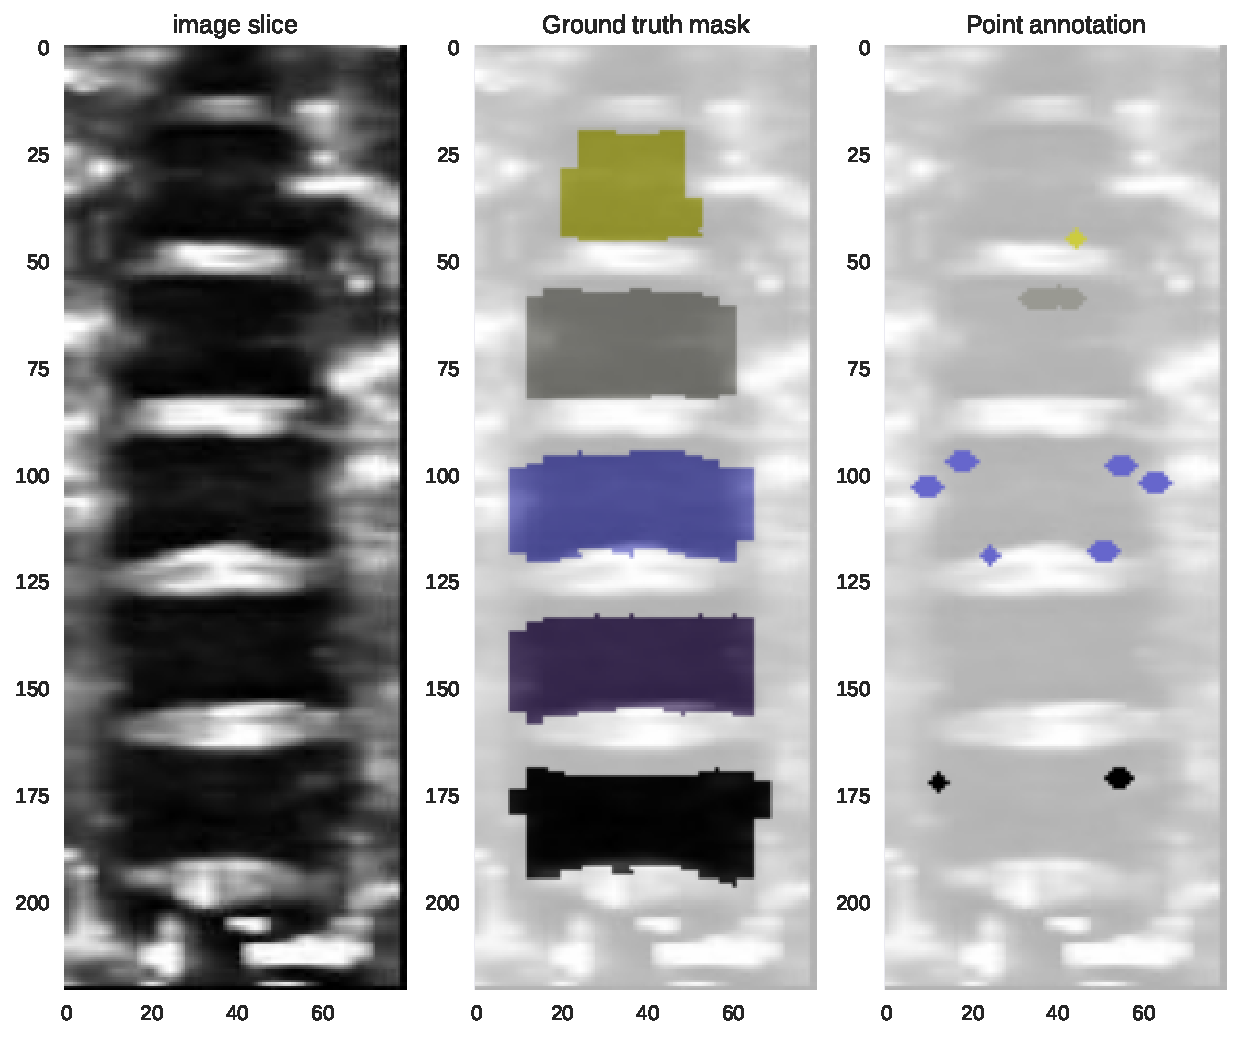
\includegraphics[width=.99\textwidth]{images/MyoSegmenTUM020_s75_front_points.pdf}
    \end{minipage} 
    \vspace{2 mm}
    \caption{Illustration of the single-stack labelling procedure.
    Since the labeller is only providing point annotations for the sagittal slices, slice 21 of MyoSegmenTUM 20 is labelled with the definded 3 class labels per class instance and 5 background point labels.
    The same annotation points show up in the frontal slice 75 of the same volume. 
    \protect\newline\noindent Colour legend: \newline
\noindent\mycircle{colL1}  L1 %\newline 
\hspace{2mm}\mycircle{colL2}  L2 %\newline 
\hspace{2mm}\mycircle{colL3}  L3 %\newline 
\hspace{2mm}\mycircle{colL4}  L4 %\newline 
\hspace{2mm}\mycircle{colL5}  L5}
\end{SCfigure}

\begin{SCfigure}[][htb]
    \centering
    \centering
    \begin{minipage}{.99\textwidth}
        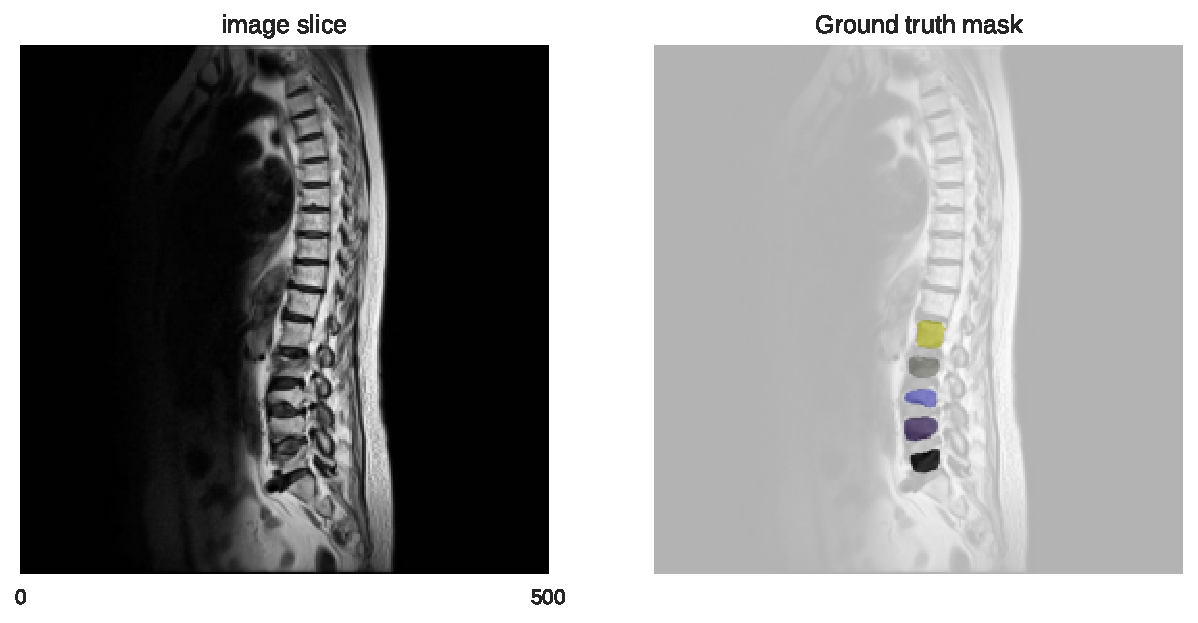
\includegraphics[width=.99\textwidth]{images/USiegen004_s20_mask.pdf}
    \end{minipage} 
    \vspace{1 mm}
    \begin{minipage}{.99\textwidth}
        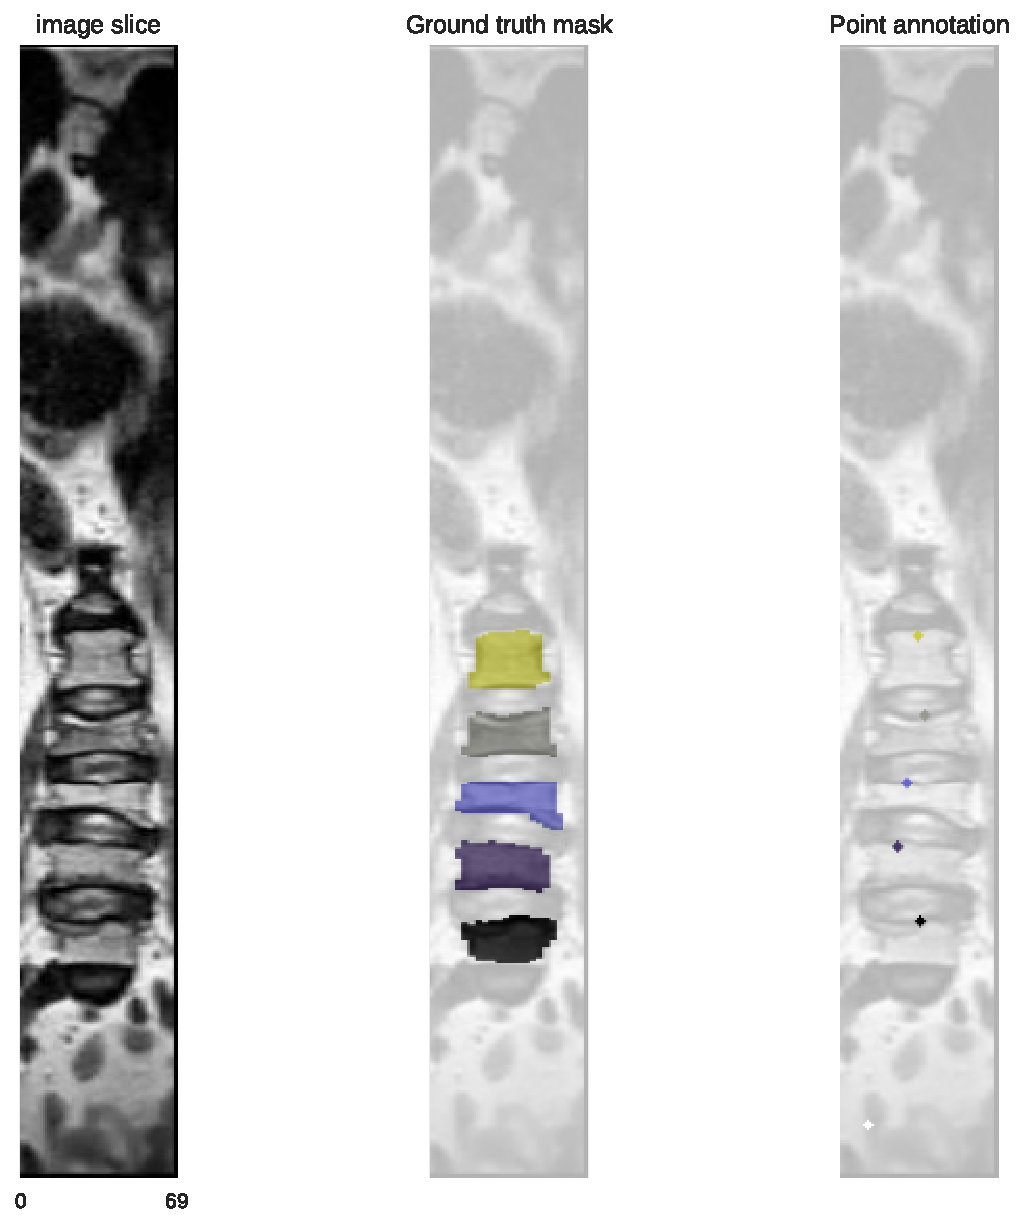
\includegraphics[width=.99\textwidth]{images/USiegen004_s250_front_points.pdf}
    \end{minipage} 
    \vspace{2 mm}
    \caption{Illustration of the single-stack labelling procedure.
    Since the labeller is only providing point annotations for the sagittal slices, slice 20 of USiegen 04 is labelled with the definded 3 class labels per class instance and 5 background point labels.
    The same annotation points show up in the frontal slice 250 of the same volume. 
    \protect\newline\noindent Colour legend: \newline
\noindent\mycircle{colL1}  L1 %\newline 
\hspace{2mm}\mycircle{colL2}  L2 %\newline 
\hspace{2mm}\mycircle{colL3}  L3 %\newline 
\hspace{2mm}\mycircle{colL4}  L4 %\newline 
\hspace{2mm}\mycircle{colL5}  L5}
\end{SCfigure}

\begin{SCfigure}[][htb]
    \centering
    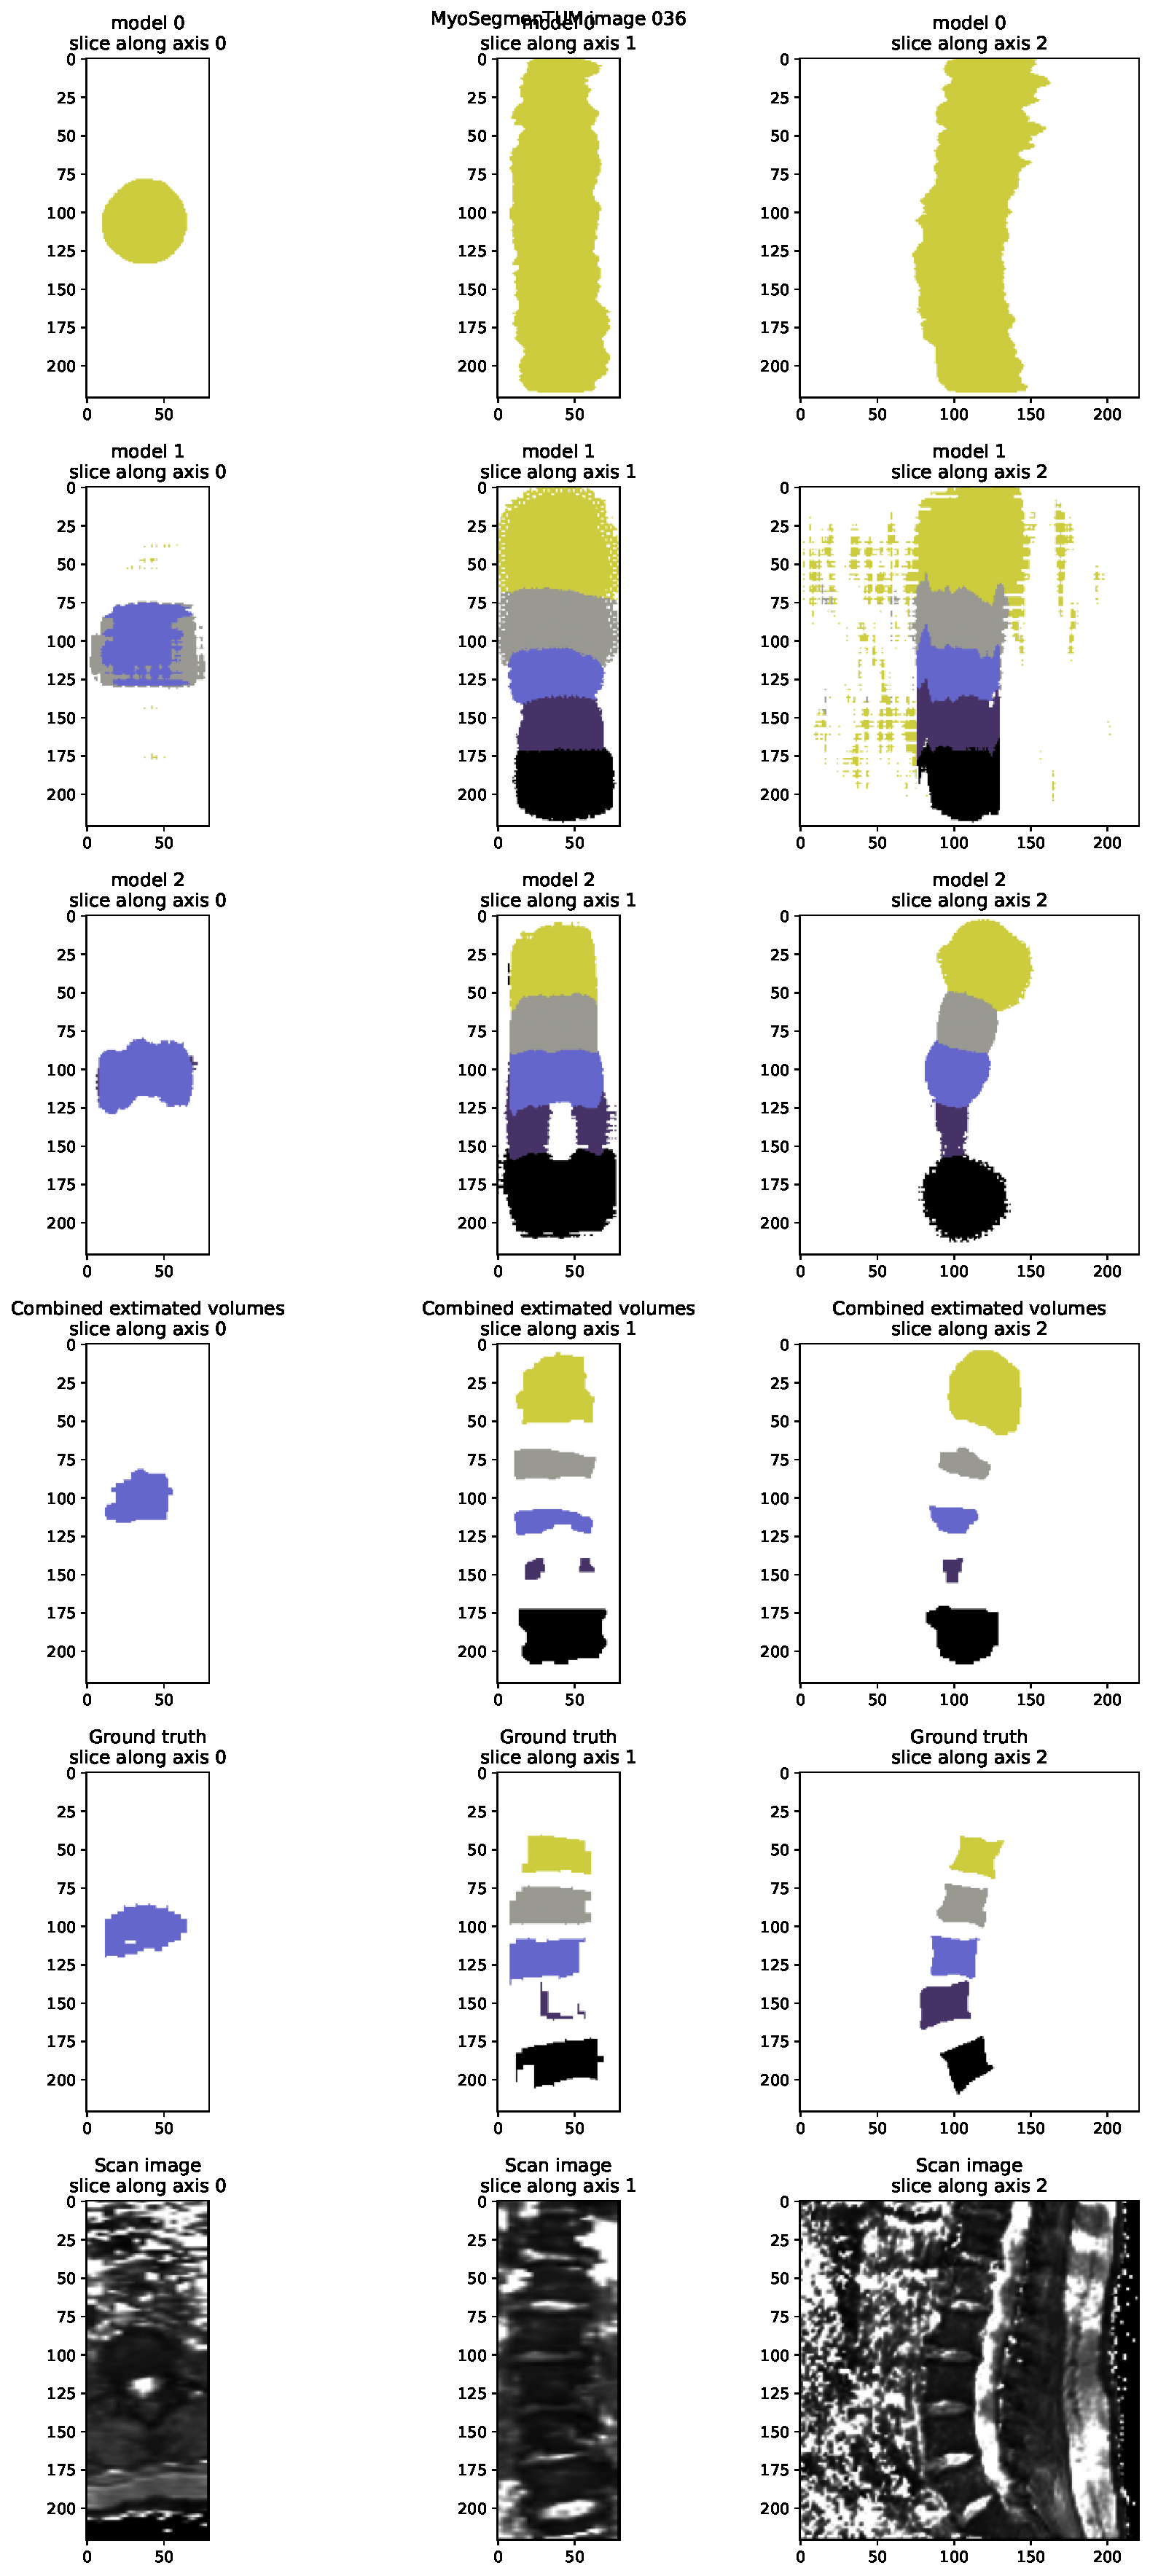
\includegraphics[width=.95\textwidth]{images/comb1_denoise2_erode1_MyoSegmenTUM_036.pdf}
    \caption{
        Result of the combination of the three single dimension model results for volume MyoSegmenTUM nr 36.
        The colours indicate the vertebra classes. Only one semantic class is estimated in the first row, illustrating the model trained on transversal slices.
        On the first three rows, slices of the resulting segmentations from the single dimension models are shown. 
        It is clear these masks contain some artefacts and are not always in agreement with each other.
        On the fourth row, the result after mask combination and morphological smoothing is shown. 
        This corresponds more closely to the ground truth mask, shown on the fifth row.
        This final mask, shown on the fourth row, will be used as a pseudo mask to approximate the unknown ground truth mask.
        In the last row, the corresponding images are shown. 
        \protect\newline\noindent Colour legend: \newline
\noindent\mycircle{colL1}  L1 %\newline 
\hspace{2mm}\mycircle{colL2}  L2 %\newline 
\hspace{2mm}\mycircle{colL3}  L3 %\newline 
\hspace{2mm}\mycircle{colL4}  L4 %\newline 
\hspace{2mm}\mycircle{colL5}  L5
        \label{fig:comb1_1}
    }
\end{SCfigure}
\begin{SCfigure}[][htb]
    \centering
    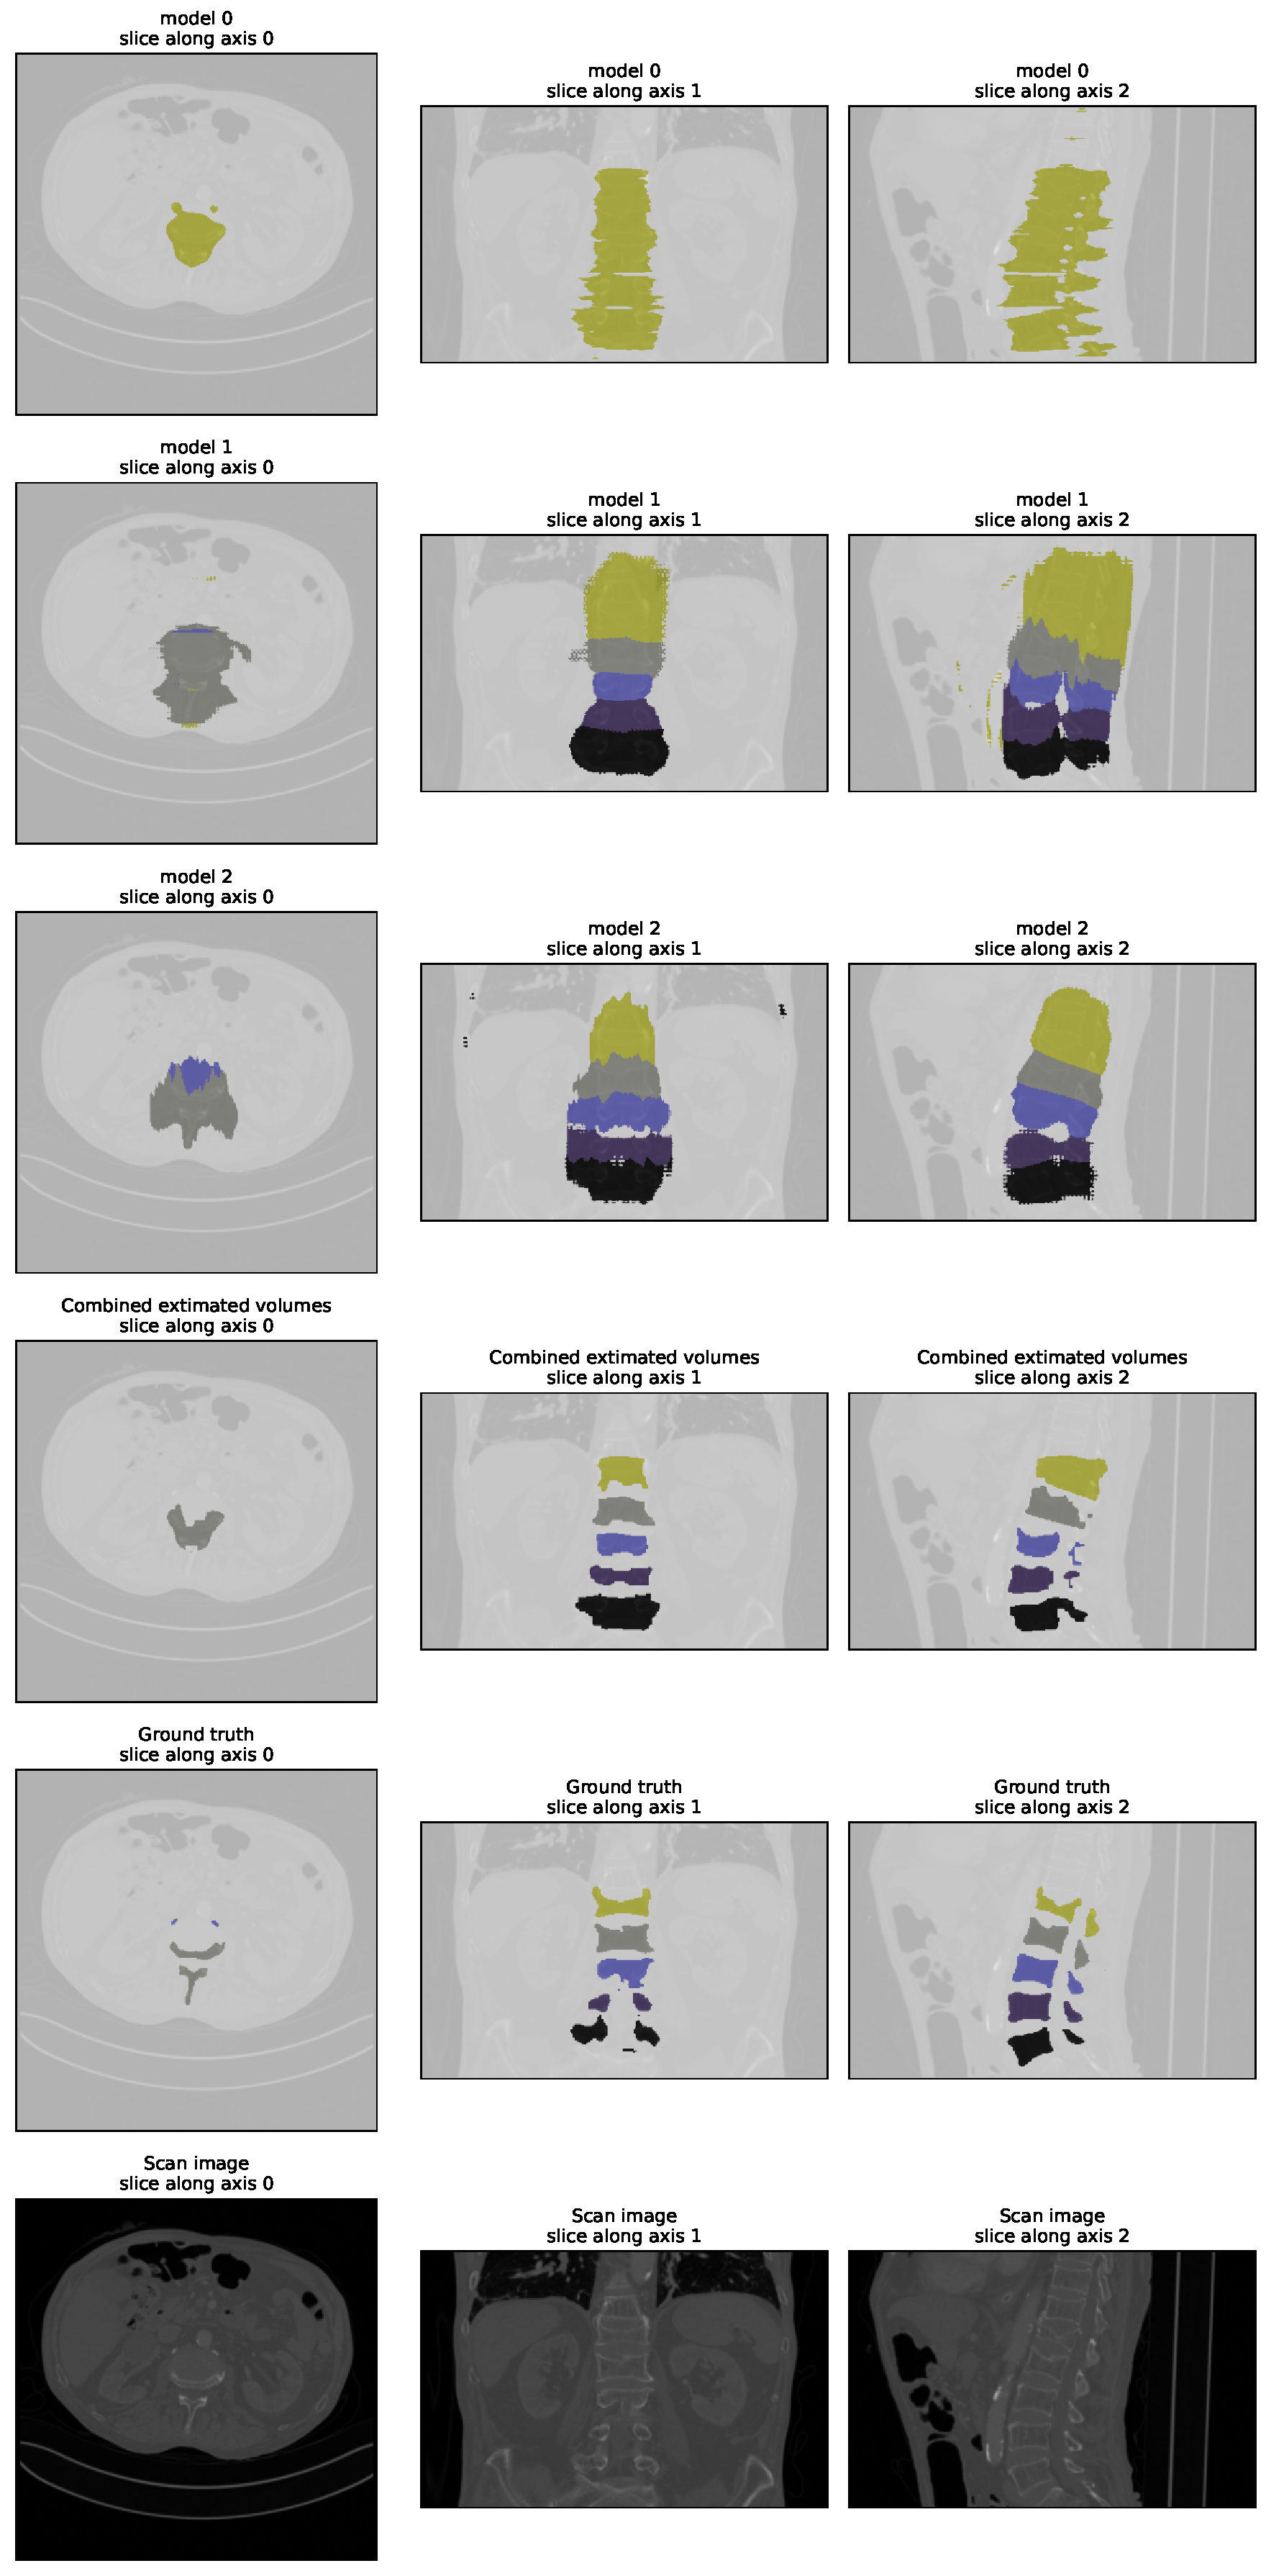
\includegraphics[width=.95\textwidth]{images/comb1_denoise2_erode1_xVertSeg_009.pdf}
    \caption{
        Result of the combination of the three single dimension model results for volume xVertSeg 009. The layout of this picture is identical to figure \ref{fig:comb1_1}.
        \protect\newline\noindent Colour legend: \newline
\noindent\mycircle{colL1}  L1 %\newline 
\hspace{2mm}\mycircle{colL2}  L2 %\newline 
\hspace{2mm}\mycircle{colL3}  L3 %\newline 
\hspace{2mm}\mycircle{colL4}  L4 %\newline 
\hspace{2mm}\mycircle{colL5}  L5
        \label{fig:comb1_2}
    }
\end{SCfigure}
\begin{SCfigure}[][htb]
    \centering
    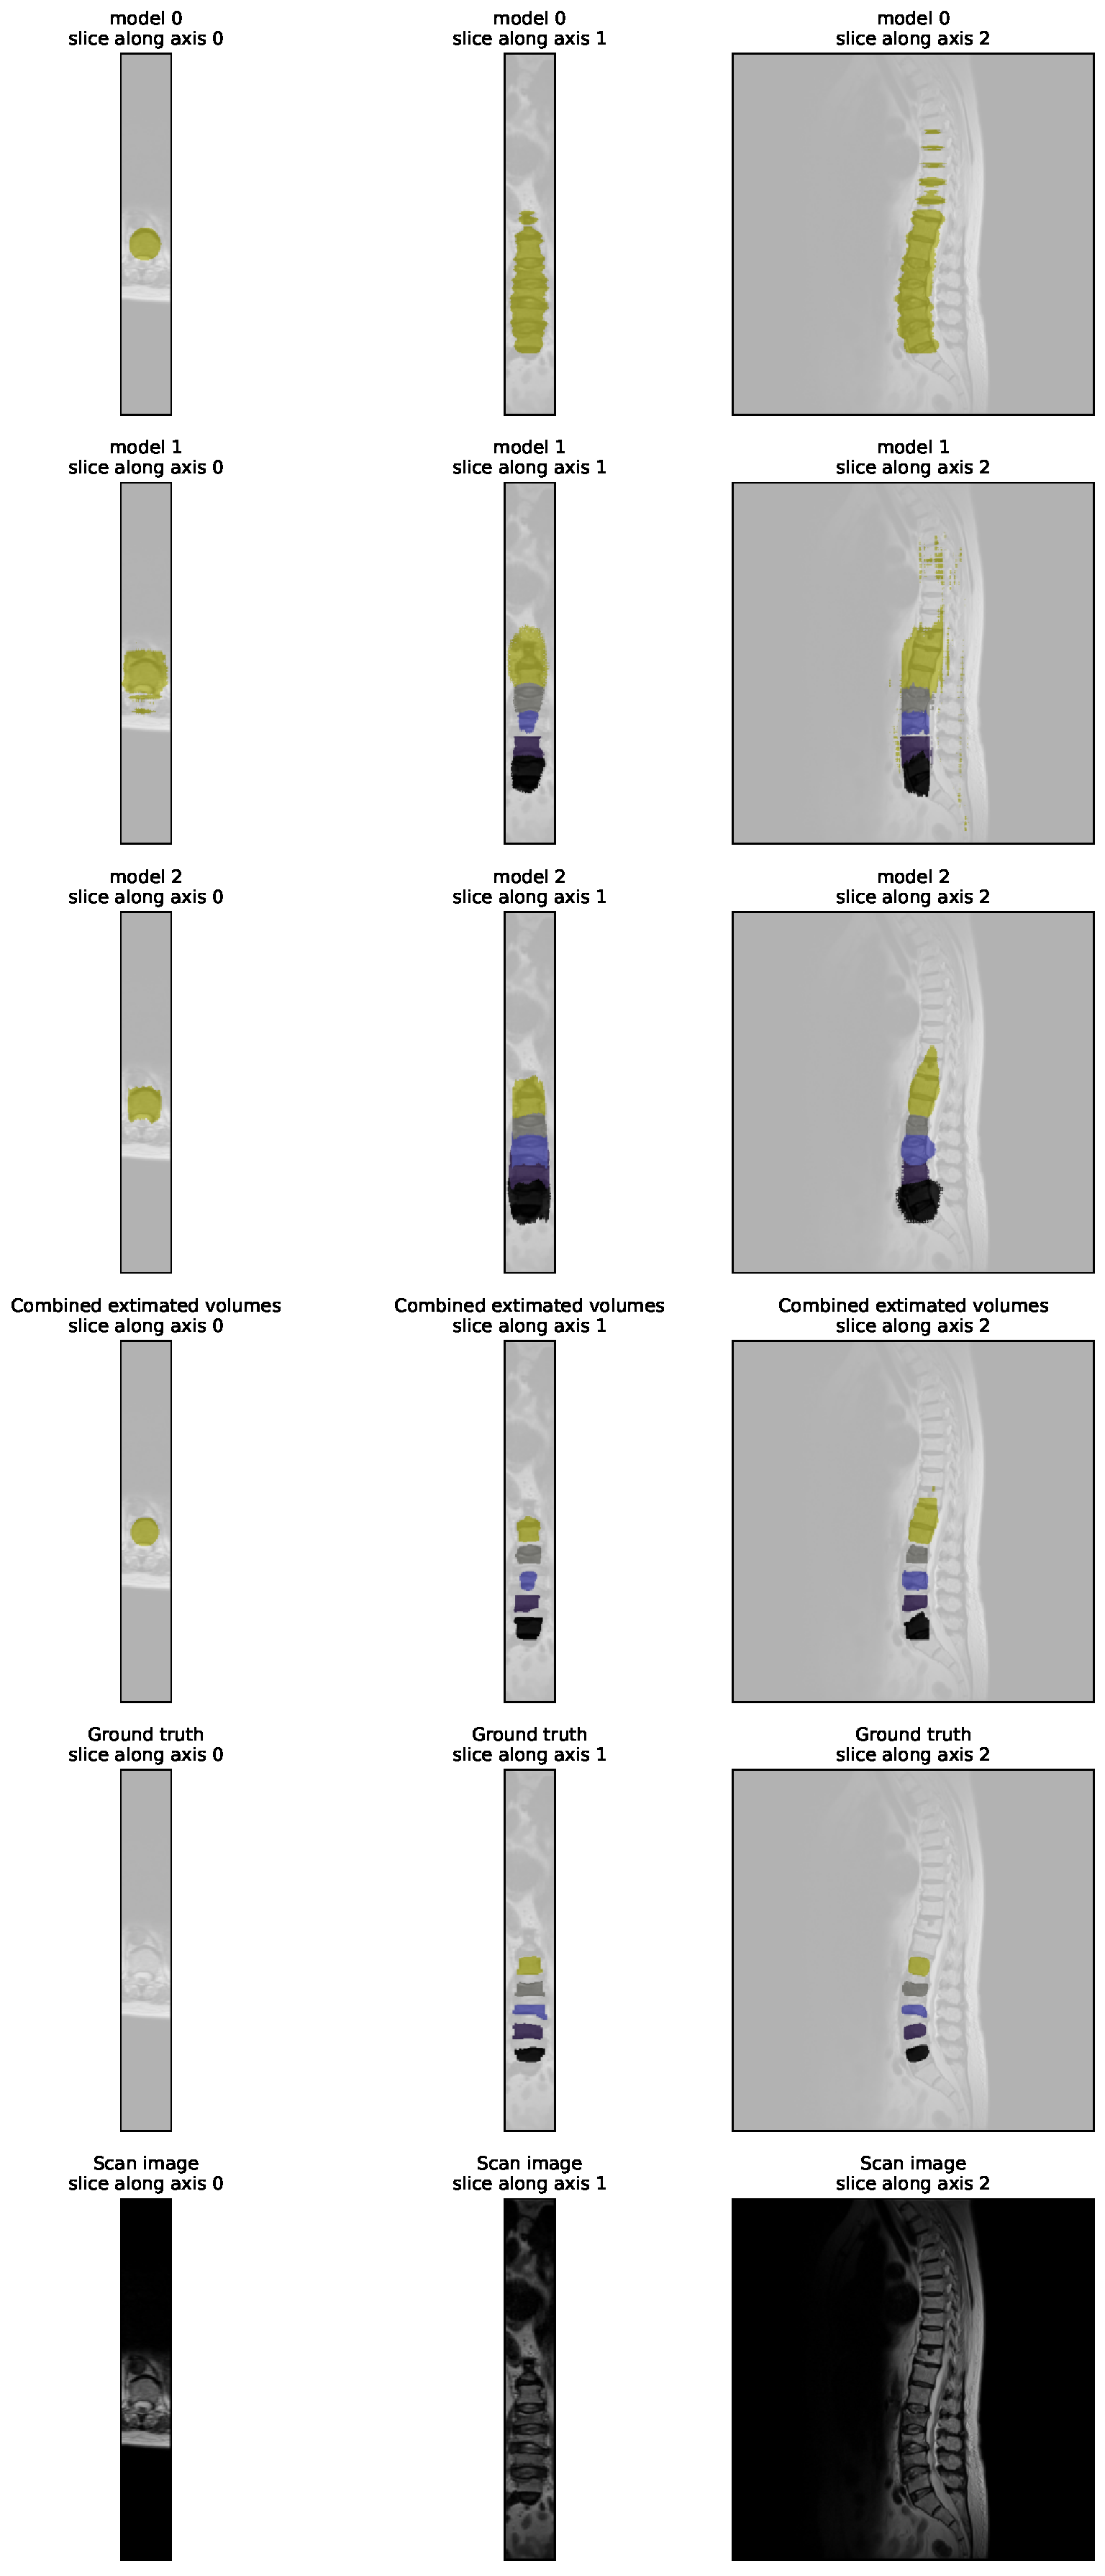
\includegraphics[width=.95\textwidth]{images/comb1_denoise2_erode1_USiegen_004.pdf}
    \caption{
        Result of the combination of the three single dimension model results for volume USiegen 004. The layout of this picture is identical to figure \ref{fig:comb1_1}.
        \protect\newline\noindent Colour legend: \newline
\noindent\mycircle{colL1}  L1 %\newline 
\hspace{2mm}\mycircle{colL2}  L2 %\newline 
\hspace{2mm}\mycircle{colL3}  L3 %\newline 
\hspace{2mm}\mycircle{colL4}  L4 %\newline 
\hspace{2mm}\mycircle{colL5}  L5
        \label{fig:comb1_3}
    }
\end{SCfigure}

\chapter{Pseudo mask training}
\marginpar{
        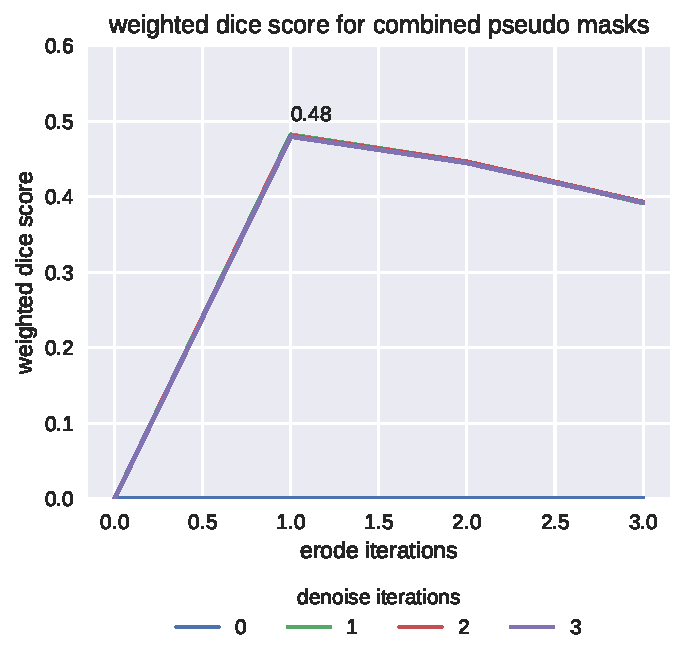
\includegraphics[width=5cm]{images/combination_optimization_precalc.pdf}
        \captionof{figure}{Illustration of the hyperparameter optimization procedure (see also table \ref{tab:combination_precalc})}
        \label{fig:hyperparameter_combination_precalc}
    }
\par{
    As described in chapter \ref{sec:annotationPoints} on page \pageref{sec:annotationPoints}, only one stack of slices will be annotated by the expert.
    This means that for the slices along one of the geometric dimensions, a known number of annotation points will be provided.
    For the slices perpendicular to the other two geometric axis, the annotation points will have to be deduced from this original stack.
}
\par{
    In this final results chapter, the following experiment is discussed:

}

\begin{SCfigure}[][htb]
    \centering
    \centering
    \begin{minipage}{.99\textwidth}
        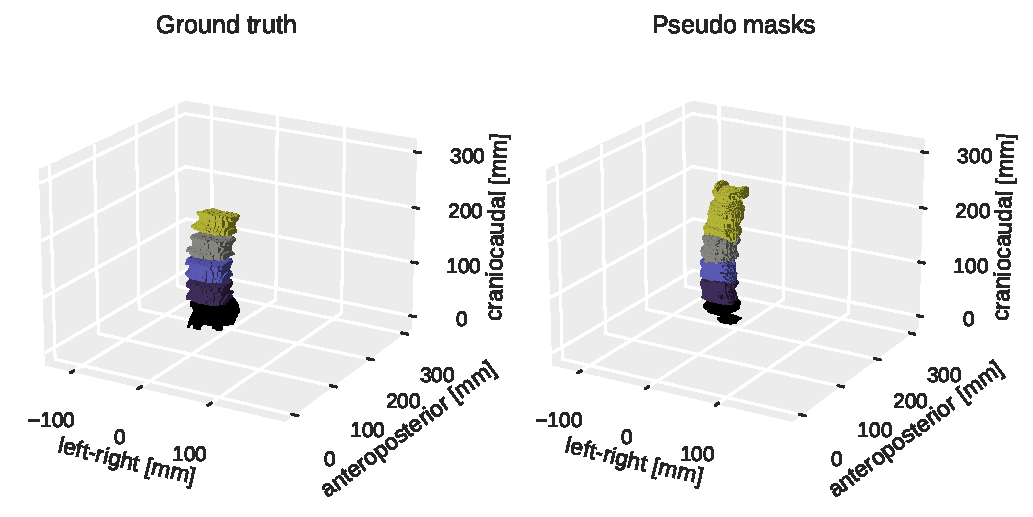
\includegraphics[width=.99\textwidth]{images/GroundTruth_morphComb_USiegen_007.pdf}
    \end{minipage} 
    \vspace{1 mm}
    \begin{minipage}{.99\textwidth}
        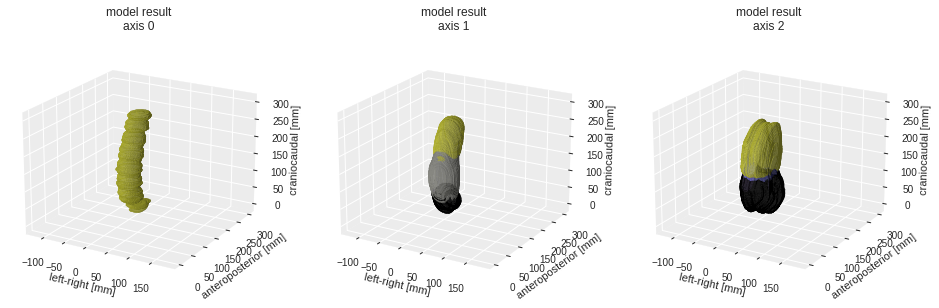
\includegraphics[width=.99\textwidth]{images/SingleDims_USiegen_007.pdf}
    \end{minipage} 
    \vspace{2 mm}
    \caption{Thee dimensional render to visualize the combination of single-dimensional model results to form the pseudo masks.
    The upper two figures show the ground truth volumes (as a reference, not used in training) and the pseudo mask volumes which have been constructed by comining the results of the three single dimensional models illustrated on the bottom row of images.
    The scan illustrated here is USiegen 007.
    \protect\newline\noindent Colour legend: \newline
\noindent\mycircle{colL1}  L1 %\newline 
\hspace{2mm}\mycircle{colL2}  L2 %\newline 
\hspace{2mm}\mycircle{colL3}  L3 %\newline 
\hspace{2mm}\mycircle{colL4}  L4 %\newline 
\hspace{2mm}\mycircle{colL5}  L5}
\end{SCfigure}

\begin{SCfigure}[][htb]
    \centering
    \centering
    \begin{minipage}{.99\textwidth}
        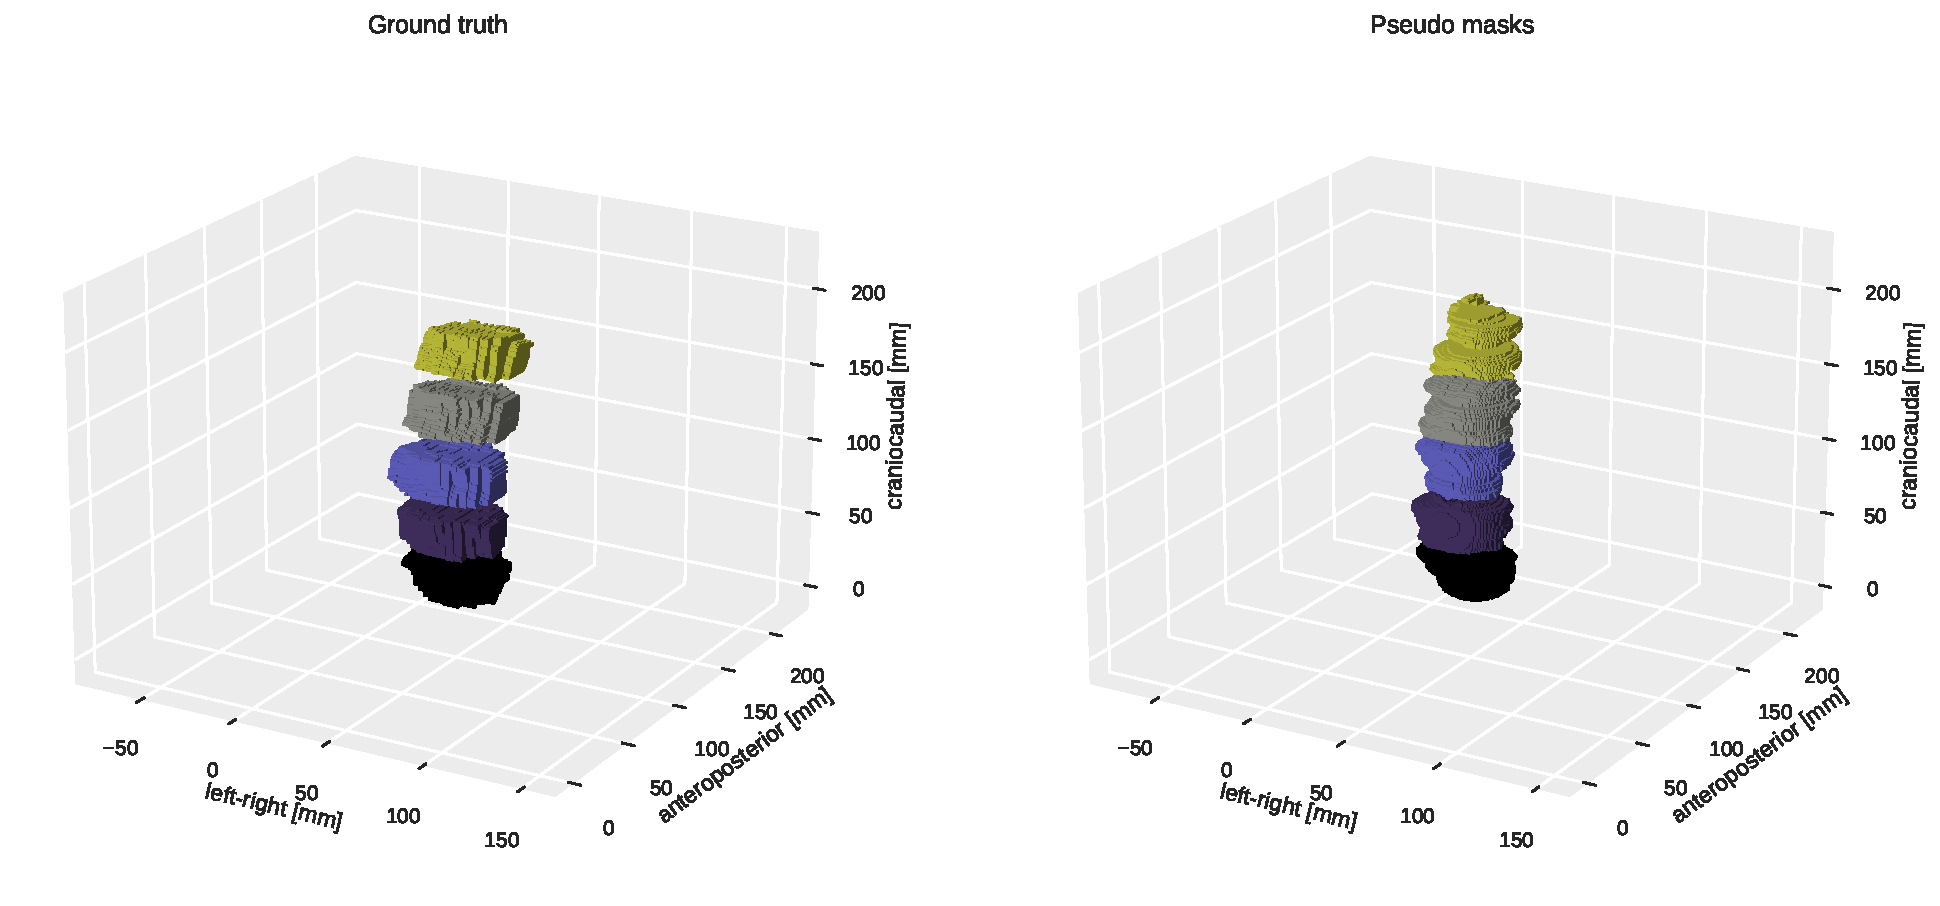
\includegraphics[width=.99\textwidth]{images/GroundTruth_morphComb_MyoSegmenTUM_034.pdf}
    \end{minipage} 
    \vspace{2 mm}
    \begin{minipage}{.99\textwidth}
        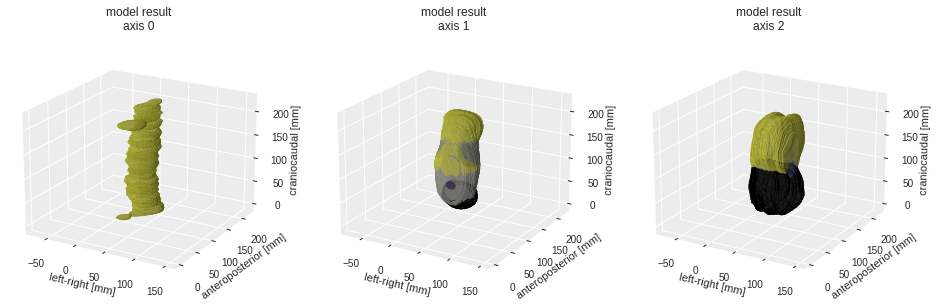
\includegraphics[width=.99\textwidth]{images/SingleDims_MyoSegmenTUM_034.pdf}
    \end{minipage} 
    \vspace{2 mm}
    \caption{Thee dimensional render to visualize the combination of single-dimensional model results to form the pseudo masks.
    The upper two figures show the ground truth volumes (as a reference, not used in training) and the pseudo mask volumes which have been constructed by comining the results of the three single dimensional models illustrated on the bottom row of images.
    The scan illustrated here is MyoSegmenTUM 34.
    \protect\newline\noindent Colour legend: \newline
\noindent\mycircle{colL1}  L1 %\newline 
\hspace{2mm}\mycircle{colL2}  L2 %\newline 
\hspace{2mm}\mycircle{colL3}  L3 %\newline 
\hspace{2mm}\mycircle{colL4}  L4 %\newline 
\hspace{2mm}\mycircle{colL5}  L5}
\end{SCfigure}


\begin{SCtable}[\sidecaptionrelwidth][h]

    \begin{tabular}{l|lll}
        \hline
        \textbf{\begin{tabular}[c]{@{}l@{}}Slice \\ direction\end{tabular}} &
          \textbf{Transverse} &
          \textbf{Coronal} &
          \textbf{Sagittal} \\ \hline
        \begin{tabular}[c]{@{}l@{}}Context\\ Slices {[}mm{]}\end{tabular}           & 1        & 1        & 1    \\ \cline{1-1}
        \begin{tabular}[c]{@{}l@{}}Points per\\ class instance\end{tabular}         & variable & variable & 3    \\ \cline{1-1}
        \begin{tabular}[c]{@{}l@{}}Background \\ points\end{tabular}                & variable & variable & 5    \\ \cline{1-1}
        Dataset &
          \begin{tabular}[c]{@{}l@{}}PLoS\\ xVertSeg\\ USiegen\\ MyoSegmenTUM\end{tabular} &
          \multicolumn{2}{l}{\begin{tabular}[c]{@{}l@{}}xVertSeg\\ USiegen\\ MyoSegmenTUM\end{tabular}} \\ \cline{1-1}
        \begin{tabular}[c]{@{}l@{}}Segmentation\\ classes\end{tabular}              & 2        & 6        & 6    \\ \cline{1-1}
        \begin{tabular}[c]{@{}l@{}}Weighted \\ dice score\end{tabular}              & 0.00     & 0.00     & 0.00 \\ \hline
        \begin{tabular}[c]{@{}l@{}}Weighted\\ dice score\\ combination\end{tabular} & \multicolumn{3}{c}{0.00}   \\ \hline
        \end{tabular}
    \caption{Combination of three point supervised models with algorithm \ref{alg:combination}. 
    These models were constructed with a fixed number of background points and a fixed number of class labels per class instance.
    This test indicates that the segmentation mask obtained from the result of single dimension models with algorithm \ref{alg:combination} allows to obtain a new segmentation mask with a higher metric score, the pseudo masks.
    The weighted dice scores are evaluated on the cross validation set, this causes the difference with the values in figure \ref{fig:points_influence}. \label{tab:combination_precalc}
    }

\end{SCtable}
\newpage

\marginpar{
        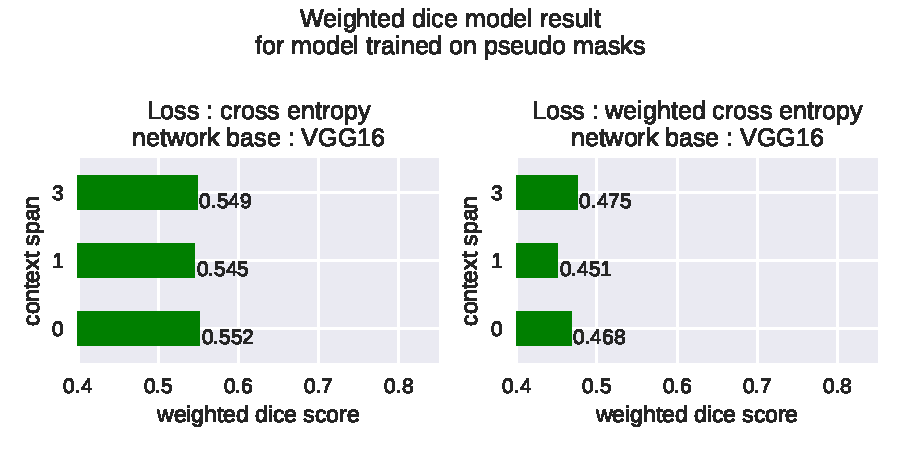
\includegraphics[width=5cm]{images/PseudoSupervised.pdf}
        \captionof{figure}{Class-weighted dice score for models trained on pseudo-masks}
        \label{fig:PseudoSupervised_dice}
    }

\todo[inline]{Time to evaluate}


\begin{SCtable}[\sidecaptionrelwidth][h]

    % Please add the following required packages to your document preamble:
% \usepackage{multirow}
\begin{tabular}{ll|lllll}
\hline
\multicolumn{2}{l}{\multirow{2}{*}{Weighted dice score}}               & \multicolumn{5}{c|}{Trained and evaluated on} \\
\multicolumn{2}{l}{} &
    all datasets &
    \begin{tabular}[c]{@{}l@{}}MyoSegmenTUM \\ only\end{tabular} &
    \begin{tabular}[c]{@{}l@{}}USiegen\\ only\end{tabular} &
    \begin{tabular}[c]{@{}l@{}}xVertSeg\\ only\end{tabular} &
    \begin{tabular}[c]{@{}l@{}}PLoS \\ only\end{tabular} \\ \hline
Reference                                                   &          & 0.76     & 0.00     & .000    & 00      &     \\ \hline
\multirow{3}{*}{\begin{tabular}[c]{@{}l@{}}Single-\\ dimension models\\ with annotation\\ poins on sagittal\\ slices\end{tabular}} &
    Transverse &
    0.53 &
    0.64 &
    0.71 &
    0.62 &
    0.70 \\
                                                            & Frontal  & 0.41     & 0.46     & 0.37    & 0.41    &     \\
                                                            & Sagittal & 0.34     & 0.36     & 0.28    & 0.36    &     \\ \hline
\begin{tabular}[c]{@{}l@{}}Pseudo mask\\ model\end{tabular} &          & 0.55     & 0.00     & 0.00    & .000    &     \\ \hline
\end{tabular}
    \caption{Summary
    }

\end{SCtable}